
\chapter{Introduction}
    (\textasciitilde2 ns)

    During the past two decades, there has been an increasing amount of new network architectures being proposed and researched. Why should we need them and what's the current state of the art in the field of network architecture?

    \section{Goals}
        The theoretical part of this thesis aims to describe alternatives to the currently prevalent network architectures. Since the Internet is by far the largest and most important example of an internetwork, its underlying architecture shall be used as a base for comparison. This is only fitting since nearly all of the network architecture research is directed towards improving the building blocks of the Internet.

        The technical report describes design and implementation of a significant part of an OMNeT++ simulation model of one of the presented architectures, RINA.

    \section{Thesis Structure}

        Part Two describes the historical events that led to the current state of the Internet and hints on the shortcomings and weak parts of current technology which create the need for an alternative architecture research.

        Part Three presents an outline of current research directions in field of network architecture and a brief overview of related research projects.

        Part Four takes a closer look at Named Data Networking, an information-centric network architecture. It contains description of the architecture and its advantages.

        Part Five takes a closer look at Recursive InterNetwork Architecture, an IPC-based network architecture. It contains description of the architecture and its advantages.

        Part Six describes implementation of Relaying and Multiplexing Task RINA in OMNeT++.

        Part Seven presents evaluation of the implementation in form of test outputs.

        Part Eight wraps it all up. ;=)

\chapter{Current State of The Internet}
    (\textasciitilde5 ns)
    The Internet could be, with no doubt, considered one of the most important technological achievements of the 20th century. It has brought a previously unimaginable degree of interconnection and information access to the whole world and its importance keeps growing even decades after its inception.

    Nevertheless,

    \section{A Brief History}
        (?? there probably won't be any space left for this)

    \section{Current Shortcomings and Weaknesses}

        \subsection{Router table size growth}

        \subsection{Node naming}

            Thus, MAC addresses and IP addresses effectively name the same thing, which is the host interface.

        \subsection{Multihoming}

            Since the IP addresses serve as point-of-attachment addresses (i.e. one per each computing system interface), there isn't any implicit mechanism for distinguishing whether multiple IP addresses belong to a single node.

        \subsection{Mobility}

        \subsection{Lack of implicit security}

        \subsection{Renumbering}

\chapter{Overview of Alternative Architectures}
    (\textasciitilde4 ns)

    This section gives an overview of paths that were pursued in the field of network architecture research.

    \section{Design Approaches}

        Over the past several years, the networking research community has exhibited many attempts of moving the field forward. The undertaken research directions are often classified into one of two groups:

        \begin{itemize}
            \item evolutionary design: backward-compatible solutions that are incrementally deployable on top of the current Internet (e.g. DiffServ, IntServ, LISP), or
            \item clean slate design: designing completely new standalone architectures that aren't constrained by Internet technology's limitations (e.g. RINA, NDN)
        \end{itemize}

        Considering the scope of this thesis, the focus will be given exclusively to "clean-slate design" architectures.

    \section{Research Initiatives}

        As designing a clean-slate architecture is an expensive and time-consuming projects, most of the research has been ...

        During the last two decades, several such initiatives have emerged, all with the same purpose: find a new technological direction for the Internet.

        Nevertheless, there are examples of lone initiatives as well.

        Projects: Named Data Networking, MobilityFirst, NEBULA, eXpressive Network Architecture, ChoiceNet

        \subsection{NewArch Project}

            DARPA-funded, nada.

        \subsection{FIRE}

            projects in 2008, 2011

        \subsection{FIBRE}

        \subsection{FIA}

            Funded by National Science Foundation.

    \section{Information-centric networking}

        \subsection{CCN}
        \subsection{NDN}
        \subsection{GreenICN}

    \section{Recursive Architectures}
        \subsection{RNA}
        \subsection{RINA}

\chapter{Named Data Networking}
    (\textasciitilde8 ns)
    \section{Premise}
        As described in section 2.1, the current Internet has its roots in telecommunication technology as this was the only area from which any inspiration could be taken. Because of this, technology of the Internet has been built on the paradigm of host-to-host communication. This can be visually presented on a "hourglass model", which indicates that while there's a wide array of technologies in use in the lower and higher layers, the hourglass's thin waist of end-to-end communication is the key static part binding different networks together.

        \begin{center}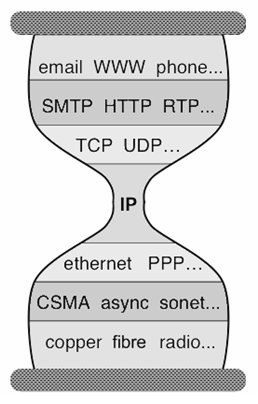
\includegraphics[width=0.2\textwidth]{media/ndn_hourglass1.jpg}\end{center}

        Building the Internet as a communication network was an obvious choice, especially since most of communication of the early ARPANET consisted of connecting terminals to mainframes and executing remote procedures on them.

        However, while the basic paradigm of host-to-host communication hasn't changed, the way we use the Internet has gone in an entirely different direction: the Internet has become mostly a content distribution network. Since the mechanism of communication over the Internet is based on creating and maintaining end-to-end connections, this creates an enormous amount of data redundancy.

        Named Data Networking proposes a solution for the problem: instead of working with the source/destination node identifiers, the "thin waist" of the Internet should work with names of data chunks.

        \begin{center}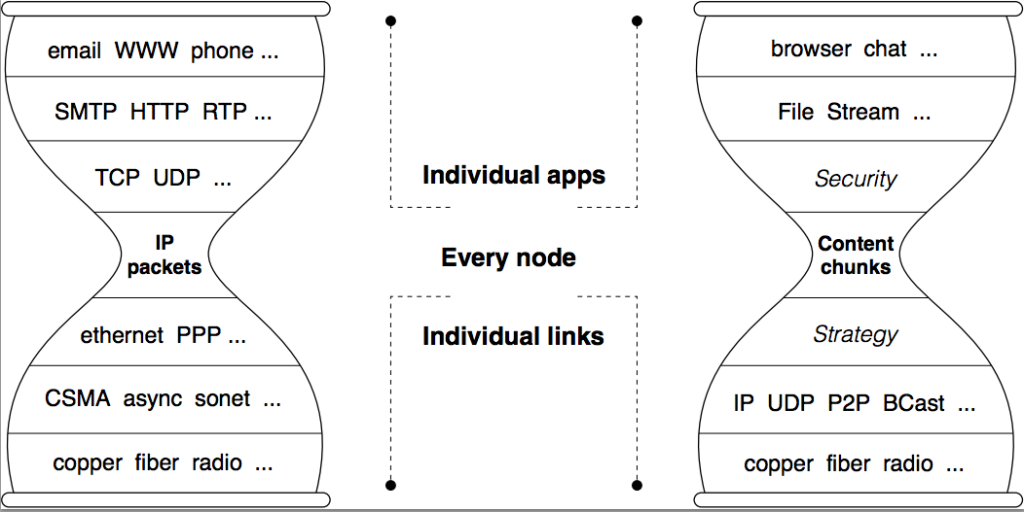
\includegraphics[width=0.6\textwidth]{media/ndn_hourglass2.png}\end{center}

    \section{Concepts}
        \subsection{The Building Blocks}
            The NDN architecture specifies:
                \begin{itemize}
                    \item two types of packets: an interest packet (containing the name of desired data) and a data packet (containing the requested data)
                \begin{center}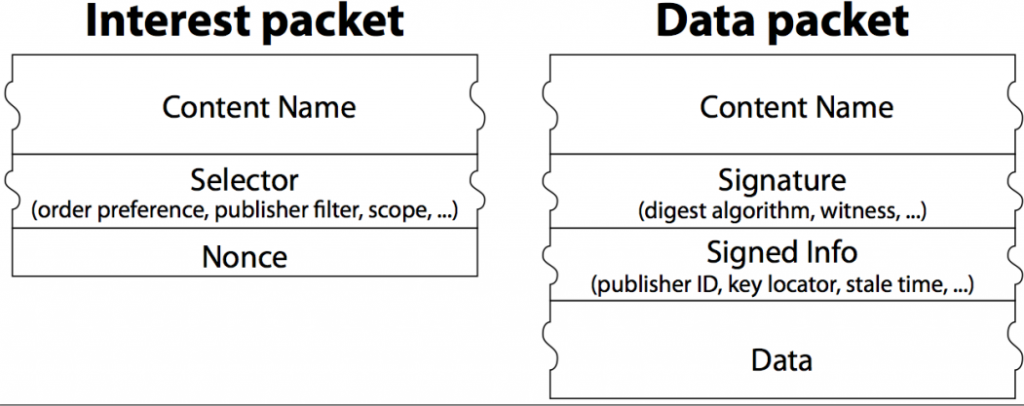
\includegraphics[width=0.6\textwidth]{media/ndn_packets1.png}\end{center}
                    \item two types of hosts: a consumer (data requester) and a producer (data provider)
                    \item a router maintaining three fundamental data structures:
                    \begin{itemize}
                        \item Forwarding Information Base (forwarding table)
                        \item Pending Interest Table (maintaining currently active requests)
                        \item Content Store (data cache)
                    \end{itemize}
                    \begin{center}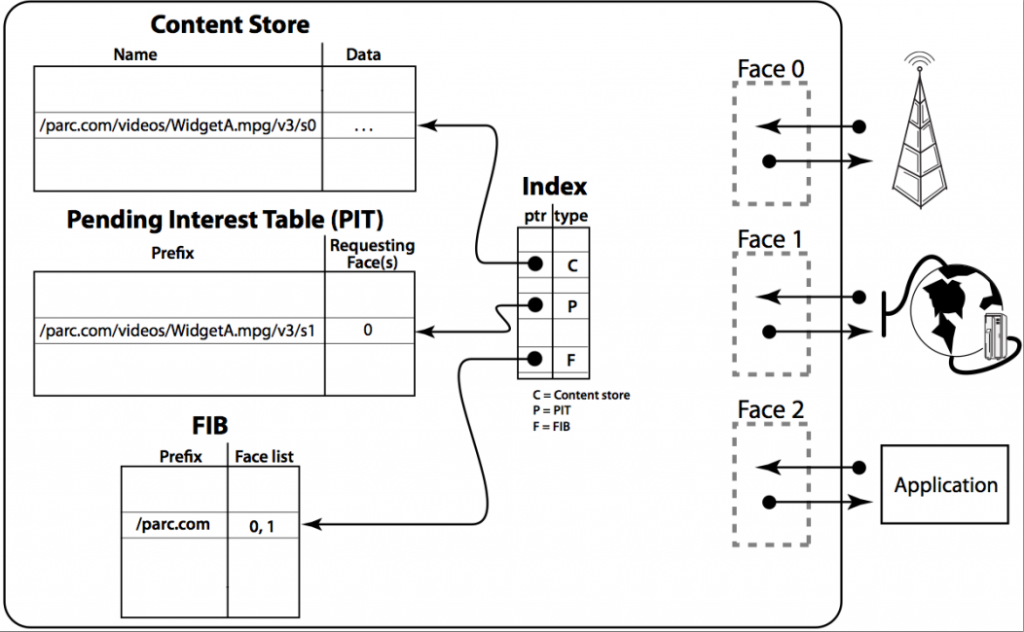
\includegraphics[width=0.6\textwidth]{media/ndn_router1.png}\end{center}

                \end{itemize}

            \subsection{The Communication Model}

            Communication in NDN is driven by the data receiver, i.e. consumer.

            \begin{enumerate}
                \item The consumer sends out an "interest packet" containing the name of the desired data.
                \item When a router receives the interest packet, it first consults its Content Store for requested data.
                    \begin{itemize}
                        \item If the data requested by the interest packet are present, they are returned in the direction of the requesting interface.
                        \item Otherwise, it'll look up the Pending Interest Table.
                        \begin{itemize}
                            \item If there's an entry present for the named data request, the entry is updated by adding the originating interface into the list of requesting interfaces, thus aggregating the new request together with an existing one.
                            \item Otherwise, a new entry is inserted, a FIB lookup is made and the interest packet is forwarded to interface(s) returned by the FIB.
                        \end{itemize}
                    \end{itemize}
                \item A data packet is returned to the router by either the producer or another router with cached data. The router finds a matching PIT entry and forwards the data to all interfaces listed in the PIT entry. The PIT entry is then removed and data are cached into the Content Store.
            \end{enumerate}

    \section{Implications}
        \subsection{Data Caching}
            The most significant feature of NDN is its native support for caching all sorts of data inside the network itself. While this should be beneficial mostly for static data such as web pages and images, dynamic content could take advantage of this as welll in case of multicasting or packet retransmission on packet loss.

        \subsection{Routing and Forwarding}
            NDN routes and forwards packets on names, which eliminates four problems caused by address forwarding in the IP architecture: address space exhaustion, NAT traversal, mobility, and address management.
            \begin{itemize}
                \item There is no address exhaustion problem since the namespace is unbounded.
                \item There is no NAT traversal problem since a host does not need to expose its address in order to offer content.
                \item Mobility, which requires changing addresses in IP, no longer breaks communication since data names remain the same.
                \item Finally, address assignment and management is no longer required in local networks, which is especially empowering for embedded sensor networks.
            \end{itemize}

            Since the forwarding mechanism otherwise bears a strong resemblance to the forwarding mechanism in IP networks, lot of the existing research on IP routing could be applied to NDN as well: protocols like BGP, IS-IS or OSPF can be, for the most part, reused with minor modifications (e.g. routers would announce name prefixes instead of IP prefixes).

        \subsection{Security}
            While TCP/IP with its end-to-end communication paradigm relies on setting up a secure channel between two hosts and transmitting data through it, NDN requires each data chunk to be signed together with its name. Thus, since security is built into the data itself, there's no need for a direct host-to-host secure channel to be created.

    \section{Current State of Implementation}

\chapter{Recursive InterNetwork Architecture}
    (\textasciitilde8 ns)
    \section{Premise}
        In 2008, computer scientist John D. Day has published a book that marked the culmination of his long-time goal of rediscovering the way we think about computer networks. The book was called Patterns in Network Architecture and in it, Day singlehandedly proposed a clean-slate approach to computer architecture that aims to get rid of most of TCP/IP's drawbacks.

        The book can be roughly divided into two separate parts: in the first part, Day attempts to decompose mechanisms used in TCP/IP to their basic parts and put them into historical and socio-economical context. He eventually discovers that the currently prevalent layered approach to network architecture is needlesly complex, because each layer consists of the same mechanisms acting on a different scope.

        The second part takes into account all of the facts discovered in the first part and uses them as foundations to build an entirely new concept of network architecture from scratch: the recursive IPC model (originally Network IPC Architecture, NIPCA).

        RINA (Recursive InterNetwork Architecture) is a currently researched network architecture based on fundamental principles described by Day.

    \section{Concepts}
        \subsection{Error And Flow Control Protocol}
        \subsection{Relaying and Multiplexing Task}
    \section{Implications}
    \section{Current State of Implementation}

\chapter{Implementation of Relaying and Multiplexing Task}
    (\textasciitilde10 ns)
    \section{OMNeT++}
        OMNeT++ is an open-source discrete simulation framework used primarily in the field of network simulation. In this context, the term "network" refers to the more general meaning of the word, which means the framework can be used not only for simulation of TCP/IP networks (especially in conjecture with the INET library), but it also provides means for simulating other networked systems such as on-chip networks or queuing networks. As we're implementing a clean-slate architecture from the ground up, this is an ideal approach.

        OMNeT++ provides a component architecture for models. Components (modules) are programmed in C++, then assembled into larger components and models using the high-level language NED. In theory, there are no limits for networks modelled by NED and the only constraint is given by a computing platform processing power.

    \section{RINASim}
        RINASim, developed by networking research group at Faculty of Information Technology of Brno University of technology, is an OMNeT++ library developed for project PRISTINE. The purpose of the library is to provide a framework for building RINA networks. RINASim is used primarily by other PRISTINE researchers to experiment with the architecture and efficiently evaluate their working theories.

    \section{Implementation Design}

        In RINASim, all functionality of RMT including a policy architecture is encompassed in a single compound module named "RelayAndMux" which is present in every IPC process. The module serves for (de)multiplexing, relaying and aggregating PDUs of data flows traversing the IPC processes.

        \subsection{Separation of mechanism and policy}
            Some aspects of RMT functionality such as queue scheduling and performance monitoring are, by their nature, suited for separation of mechanism and policy. In another words, we need to take into account that architecture implementators will probably want to specify custom behavior for some of the logic present in RMT.

            For this purpose, several algorithms used by RMT are meant to be user-configurable:

            \begin{itemize}
                \item RMT scheduling policy: The scheduling algorithm that determines the order input and output buffers are serviced (e.g. by number of waiting PDUs in buffers or with fair queuing).
                \item RMT monitoring policy: A queue monitoring algorithm that is invoked each time a PDU enters or leaves a queue. This policy should compute variables (such as average queue length) to be used in decision process of other policies.
                \item RMT maxqueue policy: An algorithm that is invoked each time a number of PDUs waiting in a queue exceeds the queue's threshold. This policy is mostly used for congestion control mechanisms (e.g. by dropping or marking the last PDU in a queue).
            \end{itemize}

        \subsection{Module structure}

            (the nasty guts of RelayAndMux.png)

            RMTModule consists of multiple simple modules of various types, some of which are instantiated only dynamically at runtime.

            Static modules:
            \begin{itemize}
                \item RMT, the central logic of Relaying And Multiplexing task that decides what should be done with messages passing through the module.
                \item RMTModuleAllocator, a control unit providing an API for adding and deleting instances of dynamic modules (RMTQueue, RMTPort).
                \item SchedulingPolicy, a scheduling policy of an RMT instance.
                \item MonitorPolicy, a monitoring policy of an RMT instance.
                \item MaxQPolicy, a maxqueue policy of an RMT instance.
            \end{itemize}

            Dynamic modules:
            \begin{itemize}
                \item RMTPort, a representation of one endpoint of an (N-1)-flow.
                \item RMTQueue, a representation of either input or output queue. The number of RMTQueues per RMTPort is determined by Resource Allocator policies.
            \end{itemize}




\chapter{Testing and Evaluation}
    (\textasciitilde4 ns)

\chapter{Conclusion \& Future Development}
    (\textasciitilde1 ns)
